% begin module trig-substitutions-ex3
\begin{frame}
\begin{example} %[Example 3, p. 505]
\begin{columns}[c]
\column{.4\textwidth}
Find $\int \frac{1}{x^2 \sqrt{x^2+4}}\diff x$.
\begin{itemize}
\item<2->  Let \alert<handout:0| 3-4,7,14,20>{$x = \uncover<4->{2\tan \theta}$}\uncover<4->{, where \alert<handout:0| 10>{$-\pi /2 \leq \theta \leq \pi / 2$}.}
\item<2->  Then \alert<handout:0| 5-6,13>{$\diff x = \uncover<6->{2\sec^2 \theta\diff \theta}$}\uncover<6->{.}
\end{itemize}
\column{.6\textwidth}
\begin{center}
\psset{xunit=2cm, yunit=2cm}
\begin{pspicture}(-0.15,-0.3)(2.3,1.2)
\psframe*[linecolor=white](-0.1,-0.3)(2.3,1.2)
\psline(0,0)(2, 0)(2,1)(0,0)
\psline(1.9,0)(1.9, 0.1)(2,0.1)
\fcAngle{0}{0.463648}{0.4}{$\theta$}
\uncover<handout:0|20->{
\rput[l](2.1, 0.5){$x$}
\rput[t](1, -0.1){$2$}
}
\uncover<handout:0|21->{
\rput[br](1, 0.55){$\sqrt{x^2+4}$}
}
%bounding box for pdflatex compilation:
\psline[linecolor=red!1](-0.11, -0.3 )(-0.105, -0.3)
\psline[linecolor=red!1](2.3, 1.21)(2.3, 1.205)
\end{pspicture}
%\ \only<handout:0| -19>{%
%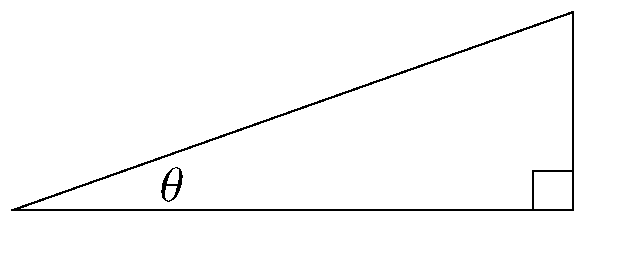
\includegraphics[height=3cm]{trig-substitution/pictures/08-03-ex3a.pdf}%
%}%
%\only<handout:0| 20>{%
%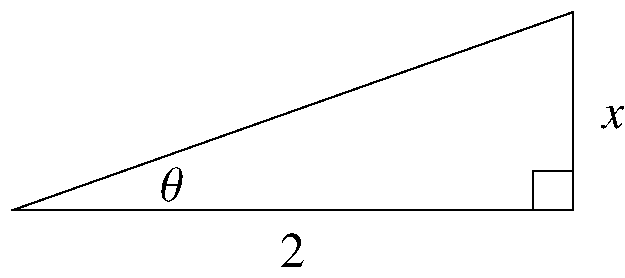
\includegraphics[height=3cm]{trig-substitution/pictures/08-03-ex3b.pdf}%
%}%
%\only<21->{%
%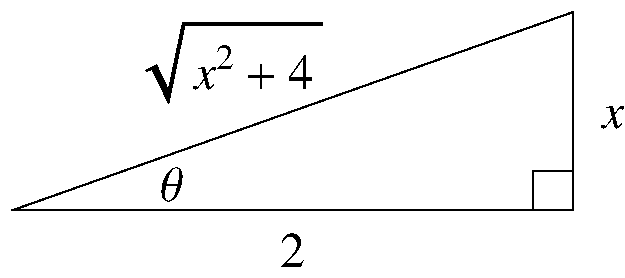
\includegraphics[height=3cm]{trig-substitution/pictures/08-03-ex3c.pdf}%
%}%
\end{center}
\end{columns}
\abovedisplayskip=0pt
\belowdisplayskip=0pt
\[
\uncover<2->{%
\alert<handout:0| 12>{%
\sqrt{\alert<handout:0| 7>{x^2} + 4} =
}%
}%
\uncover<7->{%
\sqrt{\alert<handout:0| 7>{4\tan^2 \theta} + 4} =
}%
\uncover<8->{%
\sqrt{4 \sec^2 \theta} =
}%
\uncover<9->{%
2 |\sec  \theta | =
}%
\uncover<10->{%
\alert<handout:0| 12>{%
2 \sec  \theta
}%
}%
\]
\abovedisplayskip=0pt
\belowdisplayskip=0pt
\begin{eqnarray*}
\uncover<11->{%
\int \frac{\alert<handout:0| 13>{\diff x}}{\alert<handout:0| 14>{x^2}\alert<handout:0| 12>{\sqrt{x^2+4}}}%
}%
& \uncover<11->{ = } & %
\uncover<11->{%
\int\frac{\alert<handout:0| 13>{2\sec^2 \theta \diff \theta}}{\alert<handout:0| 14>{4\tan^2 \theta}\cdot \alert<handout:0| 12>{2\sec \theta}}
}%
\uncover<15->{%
 = \frac{1}{4}\int \frac{\cos \theta}{\sin^2\theta} \diff \theta
}\\%
\uncover<16->{%
\textrm{Let } \alert<handout:0| 19>{u = \sin \theta} :%
}%
& \uncover<17->{ = } & %
\uncover<17->{%
\frac{1}{4} \int \frac{\diff u}{u^2}
}  \uncover<18->{ = }  \uncover<18->{%
\frac{1}{4} \left( -\alert<handout:0| 19>{\frac{1}{u}}\right)  + C
}\\%
& \uncover<19->{ = } & %
\uncover<19->{%
 -\frac{\alert<handout:0| 19,22-23>{\csc \theta}}{4} + C
}%
\uncover<23->{%
=  -\frac{\alert<handout:0| 23>{\sqrt{x^2+4}}}{4\alert<handout:0| 23>{x}} + C
}%
\end{eqnarray*}
\end{example}
\end{frame}
% end module trig-substitutions-ex3
